\documentclass[11pt,letterpaper]{article}

\usepackage[margin=1in,headheight=14pt]{geometry}
\usepackage{amsmath,amssymb,amsthm,mathtools}
\usepackage{graphicx}
\usepackage{tikz}
\usepackage{xcolor}
\usepackage{enumitem}
\usepackage{microtype}
\usepackage{fancyhdr}
\usepackage[colorlinks=true,linkcolor=blue,citecolor=blue,urlcolor=blue]{hyperref}

% Personal notation and theorem environments.
%!TEX root = EM_singular_models.tex

% PDF margin etc settings
%\setlength{\textwidth}{\paperwidth}
%\addtolength{\textwidth}{-6cm}
%\setlength{\textheight}{\paperheight}
%\addtolength{\textheight}{-4cm}
%\addtolength{\textheight}{-1.1\headheight}
%\addtolength{\textheight}{-\headsep}
%\addtolength{\textheight}{-\footskip}
%\setlength{\oddsidemargin}{0.5cm}
%\setlength{\evensidemargin}{0.5cm}

%%%%%%%%%%%%%%%%%%%%%%%%%%%%%%%%

% MACROS HERE

%%%%%%%%%%%%%%%%%%%%%%%%%%%%%%%%

\newcommand{\fixedpointtheta}{\widehat\theta_\obs}

\newcommand{\cover}{N}
\newcommand{\kinit}{\nu}
\newcommand{\cdelta}{c_\threshold}
\newcommand{\dndelta}{\omega}
\newcommand{\kndelta}{\Upsilon}
\newcommand{\kndeltanew}{\Psi}
\newcommand{\radii}{\mathcal{R}}
\newcommand{\event}{\mathcal{E}}
\newcommand{\kevent}{\mathcal{D}}


% Observations, dimension etc.
\newcommand{\dims}{\ensuremath{d}}
\newcommand{\samples}{\ensuremath{n}}
\newcommand{\obs}{\samples}
\newcommand{\real}{\ensuremath{\mathbb{R}}}
\newcommand{\complex}{\ensuremath{\mathbb{C}}}
\newcommand{\realdim}{\ensuremath{\real^\dims}}

\newcommand{\smallthreshold}{\epsilon}

% some mathcal notations
\newcommand{\order}[1]{\ensuremath{\mathcal{O}\parenth{#1}}}

% Basic statistics notation
\newcommand{\xstar}{\ensuremath{x^*}}
\newcommand{\xbar}{\ensuremath{\bar{x}}}
% True parameter
\newcommand{\thetastar}{\ensuremath{{\theta^*}}}
% Estimate one
\newcommand{\thetahat}{\ensuremath{\widehat{\theta}}}
% Estimate two
\newcommand{\thetatil}{\ensuremath{\widetilde{\theta}}}
\newcommand{\thetabar}{\ensuremath{\bar{\theta}}}
\newcommand{\yvec}{\ensuremath{y}}
\newcommand{\Xmat}{\ensuremath{X}}

% Distributions
\newcommand{\distribution}{P}
\newcommand{\density}{f}
\newcommand{\gaussiandensity}{\phi}
\newcommand{\NORMAL}{\ensuremath{\mathcal{N}}}
\newcommand{\BER}{\ensuremath{\mbox{Ber}}}

% Spaces
\newcommand{\Xspace}{\ensuremath{\mathcal{X}}}
\newcommand{\Yspace}{\ensuremath{\mathcal{Y}}}
\newcommand{\Zspace}{\ensuremath{\mathcal{Z}}}


% Brackets Size
\newcommand{\brackets}[1]{\left[ #1 \right]}
\newcommand{\parenth}[1]{\left( #1 \right)}
\newcommand{\bigparenth}[1]{\big( #1 \big)}
\newcommand{\biggparenth}[1]{\bigg( #1 \bigg)}
\newcommand{\braces}[1]{\left\{ #1 \right \}}
\newcommand{\abss}[1]{\left| #1 \right |}
\newcommand{\angles}[1]{\left\langle #1 \right \rangle}
\newcommand{\tp}{^\top}

% Generic vectors and scalars
\newcommand{\myvec}{u} % for generic vector
\newcommand{\myvectwo}{v} % for generic vector
\newcommand{\mymat}{B}
\newcommand{\set}{{A}}
\newcommand{\scalar}{\alpha}
\newcommand{\tvscalar}{\epsilon}
\newcommand{\tailboundscalar}{t}
\newcommand{\term}{U}
\newcommand{\myVarone}{\alpha_X}
\newcommand{\myVartwo}{\alpha_Y}
\newcommand{\myCovmat}{\Sigma}
\newcommand{\xcord}[1]{x^{(#1)}}
\newcommand{\xcordpop}[1]{X^{(#1)}}
\newcommand{\ycordpop}[1]{Y^{(#1)}}
\newcommand{\myVarthree}{\ensuremath{U}}
\newcommand{\myVarfour}{\ensuremath{V}}
\newcommand{\myfuntwo}{\ensuremath{g}}
\newcommand{\numsteps}{t}
\newcommand{\totalnumsteps}{T}
\newcommand{\seqalpha}[1]{\alpha_{#1}}
\newcommand{\seqnu}[1]{\nu^{(#1)}}
\newcommand{\imax}{\ell_\smallthreshold}
\newcommand{\basis}{e}
\newcommand{\radem}{\varepsilon}
\newcommand{\Tone}{T\ensuremath{_{0}}}
\newcommand{\Ttwo}{T\ensuremath{_{2}}}
\newcommand{\contractPar}[1]{\ensuremath{\gamma\parenth{#1}}}

\newcommand{\simiid}{\overset{\mathrm{i.i.d.}}{\sim}}
\newcommand{\eqd}{\overset{d}{=}}


% EM updates
\newcommand{\hidden}{Z}
\newcommand{\qfun}[2]{Q(#1\vert#2)}
\newcommand{\variable}{\theta}
\newcommand{\weights}{w}
\newcommand{\myfun}{q}
\newcommand{\gradf}{\nabla \myfun}
\newcommand{\hessf}{\nabla^2 \myfun}
\newcommand{\iter}{t}
\newcommand{\mupdate}{M}
\newcommand{\mupdategeneral}{\ensuremath{M^{GN}}}




% EM contractions
\newcommand{\contractgene}{\ensuremath{\gamma^{GN}}}
\newcommand{\updateMat}{\ensuremath{\Gamma_{\theta}}}
\newcommand{\mymatTheta}{\ensuremath{B_{\theta}}}
\newcommand{\sech}{\text{sech}}

% Nhat's macros 
\newcommand{\Rspace}{\ensuremath{\mathbb{R}}}
\newcommand{\Ecal}{\ensuremath{\mathcal{E}}}
\newcommand{\Ncal}{\ensuremath{\mathcal{N}}}
\newcommand{\gradient}{\ensuremath{\nabla}}
\newcommand{\smallweight}{\ensuremath{\epsilon^{sw}}}
\newcommand{\smallnorm}{\ensuremath{\rho^{sw}}}
\newcommand{\ball}{\ensuremath{\mathbb{B}}}
\newcommand{\sphere}{\ensuremath{\mathbb{S}}}

\newcommand{\diam}{\ensuremath{\text{diam}}}
\newcommand{\upper}{\ensuremath{\bar{C}}}
\newcommand{\sample}{\ensuremath{\xi}}
\newcommand{\weight}{\ensuremath{\pi}}
\newcommand{\contracasym}{\ensuremath{\rho}}
\newcommand{\Fishermatrix}{\ensuremath{\mathcal{I}}}
\newcommand{\barcontracasym}{\ensuremath{\bar{\rho}}}


\newcommand{\TrueDensity}{\ensuremath{f}}
\newcommand{\FitDensity}{\ensuremath{f}_{\theta}}
\newcommand{\FitDensityfree}{\ensuremath{f}_{\pi, \theta}}
\newcommand{\FitDensitygen}{\ensuremath{f}_{\pi, \theta_{1}, \theta_{2}}}
\newcommand{\FitDensitymore}{\ensuremath{f}_{G}}
\newcommand{\normden}{\ensuremath{\phi}}
\newcommand{\mean}{\ensuremath{\theta}}
\newcommand{\sd}{\ensuremath{\sigma}}
\newcommand{\parFOS}{\ensuremath{\gamma}}
\newcommand{\funQ}{\ensuremath{Q}}
\newcommand{\updateM}{\ensuremath{M}}
\newcommand{\weightFun}{\ensuremath{w}}
\newcommand{\mydefn}{\ensuremath{:=}}
\newcommand{\poincare}{\ensuremath{\tilde{C}}}
\newcommand{\paraspace}{\ensuremath{\Theta}}
\newcommand{\loglihood}{\ensuremath{F}}
\newcommand{\prior}{\ensuremath{\pi}}
\newcommand{\posterior}{\ensuremath{\Pi}}
\newcommand{\boundcons}{\ensuremath{B}}
\newcommand{\boundconstot}{\ensuremath{H}}
\newcommand{\noise}{\ensuremath{\varepsilon}}
\newcommand{\loglihoodgaus}{\ensuremath{F^{G}}}
\newcommand{\loglihoodind}{\ensuremath{F^{I}}}
\newcommand{\loglihoodlogit}{\ensuremath{F^{R}}}
\newcommand{\noiseone}{\ensuremath{\varepsilon_{1}}}
\newcommand{\noisetwo}{\ensuremath{\varepsilon_{2}}}

%%%SDE_Bayesian_inf
\newcommand{\weakcon}{\ensuremath{\psi}}
\newcommand{\perturb}{\ensuremath{\zeta}}
\newcommand{\inver}{\ensuremath{\xi}}

% Universal constants
\newcommand{\unicon}{c}
\newcommand{\uniconnew}{c'}
\newcommand{\uniconone}{c_1}
\newcommand{\unicontwo}{c_2}

% some parameters that you may define
\newcommand{\scparam}{m} % strong  convexity parameter
\newcommand{\smoothness}{L} % smoothness parameter
\newcommand{\step}{h}


%%%%%%%%% Distributions and Random variables %%%%%%%%%%%
\newcommand{\rvg}{\xi} % to denote the random variable g
\newcommand{\threshold}{\delta}


%%%%%%%%% Basic Terms like defn, etal, tmix, polylog %%%%%%%%%%%
\newcommand{\defn}{:=}
\newcommand{\rdefn}{=:}
\newcommand{\etal}{{et al.}}
\newcommand{\polylog}{\text{poly-log}}

% Some vector/matrix norms
\newcommand{\matnorm}[3]{|\!|\!| #1 | \! | \!|_{{#2}, {#3}}}
\newcommand{\matsnorm}[2]{|\!|\!| #1 | \! | \!|_{{#2}}}
\newcommand{\vecnorm}[2]{\left\| #1\right\|_{#2}}
\newcommand{\enorm}[1]{\vecnorm{#1}{2}} % euclidean norm
\newcommand{\nucnorm}[1]{\ensuremath{\matsnorm{#1}{\footnotesize{\mbox{nuc}}}}}
\newcommand{\fronorm}[1]{\ensuremath{\matsnorm{#1}{\footnotesize{\mbox{fro}}}}}
\newcommand{\opnorm}[1]{\ensuremath{\matsnorm{#1}{\tiny{\mbox{op}}}}}
%%% EM paper
\newcommand{\constrainnorm}[1]{\vecnorm{#1}{[k]}} % euclidean norm

\newcommand{\bigmatsnorm}[2]{{\Big|\!\Big|\!\Big| #1
  \Big|\!\Big|\!\Big|}_{#2}}

% Inner product
\newcommand{\inprod}[2]{\ensuremath{\langle #1 , \, #2 \rangle}}

% Kullback-Leibler
\newcommand{\kull}[2]{\ensuremath{D_{\text{KL}}(#1\; \| \; #2)}}

% Probability
\newcommand{\Exs}{\ensuremath{{\mathbb{E}}}}
\newcommand{\Prob}{\ensuremath{{\mathbb{P}}}}

%Eigenvector / eigenvalue related notation
\newcommand{\eig}[1]{\ensuremath{\lambda_{#1}}}
\newcommand{\eigmax}{\ensuremath{\eig{\max}}}
\newcommand{\eigmin}{\ensuremath{\eig{\min}}}

% \DeclareMathOperator{\det}{det}
\DeclareMathOperator{\modd}{mod}
\DeclareMathOperator{\diag}{diag}
\DeclareMathOperator{\var}{var}
\DeclareMathOperator{\cov}{cov}
\DeclareMathOperator{\trace}{trace}
\DeclareMathOperator{\abs}{abs}
\DeclareMathOperator{\floor}{floor}
\DeclareMathOperator{\vol}{vol}
\DeclareMathOperator{\child}{child}
\DeclareMathOperator{\parent}{parent}
\DeclareMathOperator{\sign}{sign}
\DeclareMathOperator{\rank}{rank}
\DeclareMathOperator{\toeplitz}{toeplitz}




\newtheoremstyle{named}{}{}{\itshape}{}{\bfseries}{.}{.5em}{\thmnote{#3's }#1}
\theoremstyle{named}
\newtheorem*{namedtheorem}{Lemma}

%%%%%%%
\theoremstyle{plain}

% {Theorem, Proposition, Lemma, Corollary} numbered sequentially
% throughout the paper
\newtheorem{theorem}{Theorem}
\newtheorem{proposition}{Proposition}
\newtheorem{lemma}{Lemma}
\newtheorem{claim}{Claim}
\newtheorem{corollary}{Corollary}
\newtheorem{definition}{Definition}
\newtheorem{conjecture}{Conjecture}
\newtheorem{remark}{Remark}
%%%%%%%%%%%%%%%%%%%%%%%%%%%%%%%%%%%%%%%%%%%%%%%%%%%%%%%%%%%%%%%%%%%%%%%
% WIDEBAR COMMAND
\newlength{\widebarargwidth}
\newlength{\widebarargheight}
\newlength{\widebarargdepth}
\DeclareRobustCommand{\widebar}[1]{%
  \settowidth{\widebarargwidth}{\ensuremath{#1}}%
  \settoheight{\widebarargheight}{\ensuremath{#1}}%
  \settodepth{\widebarargdepth}{\ensuremath{#1}}%
  \addtolength{\widebarargwidth}{-0.3\widebarargheight}%
  \addtolength{\widebarargwidth}{-0.3\widebarargdepth}%
  \makebox[0pt][l]{\hspace{0.3\widebarargheight}%
    \hspace{0.3\widebarargdepth}%
    \addtolength{\widebarargheight}{0.3ex}%
    \rule[\widebarargheight]{0.95\widebarargwidth}{0.1ex}}%
  {#1}}



%%% New version of \caption puts things in smaller type, single-spaced
%%% and indents them to set them off more from the text.
\makeatletter
\long\def\@makecaption#1#2{
        \vskip 0.8ex
        \setbox\@tempboxa\hbox{\small {\bf #1:} #2}
        \parindent 1.5em  %% How can we use the global value of this???
        \dimen0=\hsize
        \advance\dimen0 by -3em
        \ifdim \wd\@tempboxa >\dimen0
                \hbox to \hsize{
                        \parindent 0em
                        \hfil
                        \parbox{\dimen0}{\def\baselinestretch{0.96}\small
                                {\bf #1.} #2
                                %%\unhbox\@tempboxa
                                }
                        \hfil}
        \else \hbox to \hsize{\hfil \box\@tempboxa \hfil}
        \fi
        }
\makeatother



%% COMMENTING commands

\long\def\comment#1{}
\definecolor{battleshipgrey}{rgb}{0.52, 0.52, 0.51}
\definecolor{darkgray}{rgb}{0.66, 0.66, 0.66}
\definecolor{darkgreen}{rgb}{0.0, 0.2, 0.13}
\definecolor{darkspringgreen}{rgb}{0.09, 0.45, 0.27}
\definecolor{dukeblue}{rgb}{0.0, 0.0, 0.61}
\definecolor{olivedrab7}{rgb}{0.24, 0.2, 0.12}
\definecolor{darkblue}{rgb}{0.0, 0.0, 0.55}
\definecolor{darkscarlet}{rgb}{0.34, 0.01, 0.1}
\definecolor{candyapplered}{rgb}{1.0, 0.03, 0.0}
\definecolor{ao(english)}{rgb}{0.0, 0.5, 0.0}
\definecolor{applegreen}{rgb}{0.55, 0.71, 0.0}

\newcommand{\red}[1]{\textcolor{red}{#1}}
\newcommand{\mjwcomment}[1]{{\bf{{\red{{MJW --- #1}}}}}}
\newcommand{\mwlcomment}[1]{{\bf{{\color{orange}{{Wenlong --- #1}}}}}}

\newcommand{\blue}[1]{\textcolor{blue}{#1}}
\newcommand{\green}[1]{\textcolor{green}{#1}}
\newcommand{\highlight}[1]{\textcolor{applegreen}{#1}}

% comment lines
\newcommand{\genecomment}[1]{{\bf{{\blue{{TEAM --- #1}}}}}}
\newcommand{\rrdcomment}[1]{{\bf{{\blue{{RRD --- #1}}}}}}
\newcommand{\nhcomment}[1]{{\bf{{\blue{{NH --- #1}}}}}}
\newcommand{\kkcomment}[1]{{\bf{{\darkgreen{{KK --- #1}}}}}}


\newcommand{\widgraph}[2]{\includegraphics[keepaspectratio,width=#1]{#2}}


\newcommand{\coursenumber}{STA3000F}
\newcommand{\coursetitle}{Advanced Theory of Statistics}
\newcommand{\courseterm}{Fall 2026}
\newcounter{lecture}
\setcounter{lecture}{8}
\newcommand{\lecturenumber}{\arabic{lecture}}
\newcommand{\lecturedate}{November 6, 2026}
\newcommand{\lecturer}{Wenlong Mou}

\pagestyle{fancy}
\fancyhf{}
\fancyhead[L]{\coursenumber: \coursetitle}
\fancyhead[R]{Lecture \lecturenumber}
\fancyfoot[C]{\lecturenumber--\arabic{page}}
\renewcommand{\headrulewidth}{0.4pt}
\renewcommand{\footrulewidth}{0pt}

\usepackage{bm}

\renewcommand{\thepage}{\lecturenumber--\arabic{page}}

\newtheorem{example}{Example}
\numberwithin{theorem}{lecture}
\numberwithin{proposition}{lecture}
\numberwithin{lemma}{lecture}
\numberwithin{claim}{lecture}
\numberwithin{corollary}{lecture}
\numberwithin{definition}{lecture}
\numberwithin{conjecture}{lecture}
\numberwithin{remark}{lecture}
\numberwithin{example}{lecture}
\numberwithin{equation}{lecture}
\counterwithin*{section}{lecture}
\renewcommand{\theHsection}{\arabic{lecture}.\arabic{section}}

\newcommand{\makelecturenotesheader}{%
  \noindent
  \textbf{\coursenumber: \coursetitle}%
  \hfill
  \textbf{\courseterm}

  \begin{center}
    {\Large\bfseries Lecture \lecturenumber: \lecturedate}
  \end{center}

  \noindent
  \textbf{Lecturer:} \lecturer
  \par\medskip
  \hrule
  \bigskip
}

\begin{document}

\makelecturenotesheader
\section{Fat-shattering dimension}
How about a function class with infinite VC dimension? In the worst case, an infinite VC dimension function class can shatter any finite set of points, and hence the covering number is unbounded. However, some classes still have structures, e.g.,
\begin{align*}
 \mathcal{F} = \Big\{ f: [0, 1] \to [0, 1] \big| |f (x) - f (y)| \leq |x - y|, \forall x, y \Big\}.
\end{align*}
This is a classical example of nonparametric estimation, and we know that we can estimate functions in this class at a rate of $n^{-1/3}$. So probably there is some structure in this function class that allows us to bound its covering number. For the subgraph class, consider the grid $x_i=i/n$ with common threshold $t_i=1/2$.

\begin{figure}[!htbp]
  \centering
  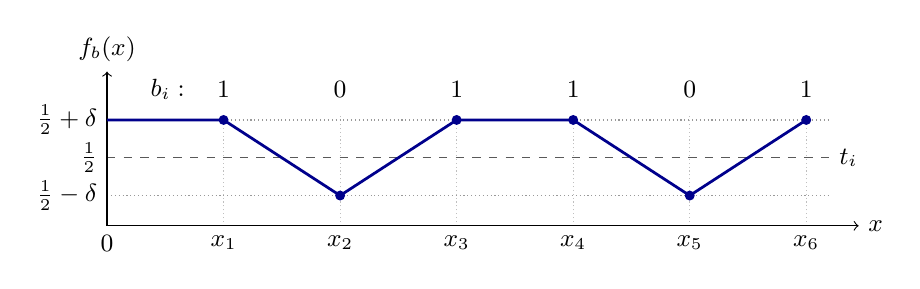
\begin{tikzpicture}[x=1.48cm,y=0.48cm,font=\small]
    \foreach \i in {1,...,6} {
      \draw[black!25,densely dotted] (\i,-1.8) -- (\i,1.15);
      \node[below] at (\i,-1.8) {$x_{\i}$};
    }
    \draw[black!40,densely dotted] (0,1) -- (6.2,1);
    \draw[black!65,dashed] (0,0) -- (6.2,0);
    \draw[black!40,densely dotted] (0,-1) -- (6.2,-1);
    \draw[->] (0,-1.8) -- (6.45,-1.8) node[right] {$x$};
    \draw[->] (0,-1.8) -- (0,2.28) node[above] {$f_b(x)$};
    \node[below] at (0,-1.8) {$0$};
    \node[left] at (0,1) {$\frac12+\delta$};
    \node[left] at (0,0) {$\frac12$};
    \node[left] at (0,-1) {$\frac12-\delta$};
    \node[right] at (6.2,0) {$t_i$};
    \node at (0.52,1.8) {$b_i:$};
    \draw[blue!55!black,line width=1pt]
      (0,1) -- (1,1) -- (2,-1) -- (3,1) -- (4,1) -- (5,-1) -- (6,1);
    \foreach \i/\bit/\height in {1/1/1,2/0/-1,3/1/1,4/1/1,5/0/-1,6/1/1} {
      \fill[blue!55!black] (\i,\height) circle[radius=1.8pt];
      \node at (\i,1.8) {$\bit$};
    }
  \end{tikzpicture}
  \caption{One labeling of the grid ($n=6$, $x_6=1$). For any labeling $b$, set $f_b(x_i)=\tfrac12+\delta(2b_i-1)$ with $\delta=1/(4n)$, interpolate linearly between grid points, and extend constantly on $[0,x_1]$. Each segment has absolute slope at most $2n\delta=1/2$. The vertical scale is magnified.}
  \label{fig:lec8-lipschitz-shattering}
\end{figure}

Figure~\ref{fig:lec8-lipschitz-shattering} shows how a $1$-Lipschitz function realizes a labeling by placing its values above or below the common threshold $t_i=1/2$. The same construction works for every labeling and every $n$, so the subgraph class has infinite VC dimension. The margin $\delta$ shrinks as the grid becomes finer. This motivates the following notion:
\begin{definition}[$\varepsilon$-fat shattering]
  Consider a sequence $(x_i, t_i)_{i = 1}^n$, it is $\varepsilon$-fat shattered by $\mathcal{F}$ if for every labeling $(b_1, \ldots, b_n) \in \{0, 1\}^n$, there exists a function $f \in \mathcal{F}$ such that
  \begin{align*}
  f (x_i)\begin{cases}
    \geq t_i + \varepsilon, & b_i = 1,\\
    \leq t_i, & b_i = 0.
  \end{cases}
  \end{align*}
\end{definition}

\begin{definition}[$\varepsilon$-fat shattering dimension]
  The $\varepsilon$-fat shattering dimension of a function class $\mathcal{F}$ is defined as the largest integer $d$ such that there exists a set of $d$ points in $\mathcal{X}$ and $d$ values $\{t_1, \ldots, t_d\}$ that can be $\varepsilon$-fat shattered by $\mathcal{F}$. If no such largest integer exists, we say that the $\varepsilon$-fat shattering dimension is infinite. This is denoted as $\text{fat}_\varepsilon (\mathcal{F})$.
\end{definition}
This can be understood as a scale-sensitive version of VC dimension.

\subsection{Using fat-shattering dimension to bound covering/packing numbers}
\begin{theorem}[Mendelson--Vershynin]
  If $\mathcal{F}$ is bounded by $1$, then there exists universal constants $c_1, c_2 > 0$ such that for any $\varepsilon \in (0, 1]$, we have
  \begin{align*}
    \sup_{Q} N (\mathcal{F}; \mathbb{L}^2 (Q), \varepsilon) \leq \Big( \frac{c_1}{\varepsilon} \Big)^{c_2 \text{fat}_{c_2 \varepsilon} (\mathcal{F})}.
  \end{align*}
\end{theorem}
There is also an improved version of this result by Rudelson--Vershynin, which gives a better dependence on $\varepsilon$:
\begin{theorem}[Rudelson--Vershynin]
  Suppose that $\mathcal{F}$ is bounded by $1$, and suppose that we have $\text{fat}_\varepsilon (\mathcal{F}) \leq g (\varepsilon)$ for some function $g$ with at most polynomial growth as $\varepsilon \to 0$. Then we have
  \begin{align*}
    \sup_{Q} N (\mathcal{F}; \mathbb{L}^2 (Q), \varepsilon) \leq \exp \Big( c_1 g (c_2 \varepsilon) \Big).
  \end{align*}
\end{theorem}
In such a case, we can apply the Dudley integral bound to get
\begin{align*}
  \Exs \sup_{f \in \mathcal{F}} \big|(P_n - P) f\big| \leq c_1 \int_0^1 \sqrt{\frac{g (c_2 \varepsilon)}{n}} d \varepsilon.
\end{align*}
\begin{itemize}
  \item If VC dimension is finite, then $\text{fat}_\varepsilon (\mathcal{F})$ is bounded by a constant, and we have the same bound as before.
  \item If $\text{fat}_\varepsilon (\mathcal{F}) \leq c \varepsilon^{-\alpha}$ for some $\alpha \in (0, 2)$, then we have
  \begin{align*}
    \Exs \sup_{f \in \mathcal{F}} \big|(P_n - P) f\big| \leq c_1 \int_0^1 \sqrt{\frac{c (c_2 \varepsilon)^{-\alpha}}{n}} d \varepsilon = c_1 \sqrt{\frac{c}{n}} \int_0^1 \varepsilon^{-\alpha/2} d \varepsilon = c_1 \sqrt{\frac{c}{n}} \cdot \frac{2}{2 - \alpha}.
  \end{align*}
  \item If we can only show that $\text{fat}_\varepsilon (\mathcal{F}) \leq c \varepsilon^{-\alpha}$ for some $\alpha \geq 2$, then the integral diverges, and we can use a truncation argument to bound the empirical process supremum.
\end{itemize}

\subsection{Examples}
Consider the one-dimensional Lipschitz function class. Now suppose that $(x_i, t_i)_{i = 1}^n$ is $\varepsilon$-fat shattered by this function class. Assume without loss of generality that $x_1 < x_2 < \cdots < x_n$. For any binary sequence $(b_1, \ldots, b_n) \in \{0, 1\}^n$, we can find a function $f_b$ in the class such that
\begin{align*}
  f_b (x_i) \begin{cases}
    \geq t_i + \varepsilon, & b_i = 1,\\
    \leq t_i, & b_i = 0.
  \end{cases}
\end{align*}
Intuitively, two adjacent points $x_i$ and $x_{i + 1}$ with different labels must have a gap of at least $\varepsilon$ in their function values. If they get too close, then the Lipschitz condition will be violated.

Formally, we fix $i$, and let $f_+$ be the function that realizes the labeling $(b_1, \ldots, b_i = 0, b_{i + 1} = 1, \ldots, b_n)$, and let $f_-$ be the function that realizes the labeling $(b_1, \ldots, b_i = 1, b_{i + 1} = 0, \ldots, b_n)$. Then we have
\begin{align*}
  f_+ (x_i) \leq t_i, \quad f_+ (x_{i + 1}) \geq t_{i + 1} + \varepsilon, \quad f_- (x_i) \geq t_i + \varepsilon, \quad f_- (x_{i + 1}) \leq t_{i + 1}.
\end{align*}
On the other hand, by the Lipschitz condition, we have
\begin{align*}
  |f_+ (x_i) - f_+ (x_{i + 1})| \leq |x_i - x_{i + 1}|, \quad |f_- (x_i) - f_- (x_{i + 1})| \leq |x_i - x_{i + 1}|.
\end{align*}
Combining these inequalities, we have
\begin{align*}
  |x_i - x_{i + 1}| \geq \max \Big\{ \varepsilon + t_{i + 1} - t_i, \varepsilon + t_i - t_{i + 1} \Big\} = \varepsilon + |t_{i + 1} - t_i| \geq \varepsilon.
\end{align*}
So we have $n \leq 1 / \varepsilon$, and hence $\text{fat}_\varepsilon (\mathcal{F}) \leq 1 / \varepsilon$. This gives a bound on the covering number of the Lipschitz function class, and hence a bound on the empirical process supremum.

\section{Localization and convergence rates}
Back to our original problem: convergence rate of $M$-estimators. We analyze
\begin{align*}
  \widehat{\theta}_n \mydefn \arg\min_{\theta \in \Theta} F_n (\theta), \quad F_n (\theta) = \frac{1}{n} \sum_{i = 1}^n f_\theta (X_i),
\end{align*}
by comparing with the population version
\begin{align*}
  \theta^* \mydefn \arg\min_{\theta \in \Theta} F(\theta), \quad F(\theta) = \Exs f_\theta ( X).
\end{align*}
We used the bound
\begin{align}
  F (\widehat{\theta}_n) - F(\theta^*) \leq 2 \sup_{\theta \in \Theta} |F_n (\theta) - F(\theta)|.\label{eq:lec8-naive-bound}
\end{align}
But this bound may be loose in practice: consider a finite-dimensional parametric model $\Theta$, leading to an empirical process bound
\begin{align*}
   \Exs \sup_{\theta \in \Theta} |F_n (\theta) - F(\theta)| \leq c \sqrt{\frac{d}{n}}.
\end{align*}
In many problems, assuming smoothness assumptions and non-degeneracy at $\theta^*$, locally, we have
\begin{align*}
  \mu \vecnorm{\theta - \thetastar}{2}^2 \leq F (\theta) - F (\theta^*) \leq \beta \vecnorm{\theta - \thetastar}{2}^2.
\end{align*}
(e.g. you can consider logistic regression as a canonical example)

From this, the best bound we can derive is $\vecnorm{\widehat{\theta}_n - \thetastar}{2} \leq c (d/n)^{1/4}$. This is even worse than the classical asymptotic $1/\sqrt{n}$ convergence.

The key problem here is that the bound~\eqref{eq:lec8-naive-bound} takes a worst-case supremum over the entire parameter space $\Theta$, which is too conservative. For our estimation problem, we know that $\thetahat_n$ is close to $\thetastar$, and in the end, we are interested in the gap $F_n - F$ evaluated at $\thetahat_n$ and $\thetastar$. So probably we can just take a supremum over $\Theta \cap \ball (\thetastar, r)$ for some radius $r$ that is shrinking with $n$.

At a superficial glance, this seems to be a chicken-egg problem: we want to bound $\vecnorm{\thetahat_n - \thetastar}{2}$, but we need to know the radius $r$ to take a supremum over. But this can be resolved by the following theorem.

\begin{theorem}[Localization]
  Assume that $F$ satisfies $F(\theta) - F (\thetastar) \geq \vecnorm{\theta - \thetastar}{2}^2$ for all $\theta \in \Theta$. Suppose that we have shown an empirical process bound for every $u > 0$:
  \begin{align}
    \Exs \Big[ \sup_{\theta \in \Theta \cap \ball (\thetastar, u)} |(P_n - P) (f_\theta - f_{\thetastar})| \Big] \leq \phi_n (u),
  \end{align}
  with a function $\phi_n (u)$ satisfying that $\phi_n (c u) \leq c^\alpha \phi_n (u)$ for every $u > 0$ and $c > 1$, with some $\alpha < 2$.

  Then for $r_n$ being the smallest positive number that satisfies the fixed-point relation
  \begin{align}
    \phi_n (r_n) \leq r_n^2,
  \end{align}
  for any $\delta > 0$, there exists a constant $c_\delta > 0$ (depending only on $\delta$ and $\alpha$) such that
  \begin{align}
    \Prob \Big( \vecnorm{\thetahat_n - \thetastar}{2} \geq c_\delta r_n \Big) \leq \delta.
  \end{align}
\end{theorem}
Parsing this theorem.
\begin{itemize}
  \item We use the localized and shifted class $\{f_\theta - f_{\thetastar}: \theta \in \Theta \cap \ball (\thetastar, u)\}$ instead of the original class $\{f_\theta: \theta \in \Theta\}$. Intuitively, if $f$ is somewhat smooth with respect to $\theta$, then the localized class should have smaller complexity than the original class.
  \item The convergence rate $r_n$ is determined implicitly by the fixed-point relation $\phi_n (r_n) \leq r_n^2$. This solution is known as the critical radius in the literature. The condition $\phi_n (c u) \leq c^\alpha \phi_n (u)$ is a technical condition that ensures that the solution to the fixed-point relation is well-defined.
  \item The result is a finite-sample high-probability bound. There is no limiting arguments, and $c_\delta$ does not depend on $n, r_n$ or any other problem parameters.
\end{itemize}
Proof: Starting with the error decomposition
\begin{align*}
  \vecnorm{\thetahat_n - \thetastar}{2}^2 \leq F (\thetahat_n) - F (\thetastar) &= F (\thetahat_n) - F_n (\thetahat_n) + \underbrace{F_n (\thetahat_n) - F_n (\thetastar)}_{ \leq 0} + F_n (\thetastar) - F (\thetastar)\\
  & \leq P f_{\thetahat_n} - P_n f_{\thetahat_n} + P_n f_{\thetastar} - P f_{\thetastar} \\
  &= (P - P_n) (f_{\thetastar} - f_{\thetahat_n}).
\end{align*}
We are interested in the tail probability
\begin{align*}
  \Prob \Big(\vecnorm{\thetahat_n - \thetastar}{2} \geq 2^M r_n \Big) = \sum_{j = M}^{\infty} \Prob \Big( 2^j r_n \leq \vecnorm{\thetahat_n - \thetastar}{2} < 2^{j + 1} r_n \Big).
\end{align*}
Because of the upper limit in each term, we can control the empirical process supremum only by looking at a local neighborhood of $\thetastar$.

For each term in the summation, we have
\begin{align*}
  &\Prob \Big( 2^j r_n \leq \vecnorm{\thetahat_n - \thetastar}{2} < 2^{j + 1} r_n \Big)\\
  & \leq \Prob \Big( \vecnorm{\thetahat_n - \thetastar}{2} < 2^{j + 1} r_n, ~  |(P_n - P) (f_{\thetastar} - f_{\thetahat_n})| \geq 2^{2j} r_n^2 \Big)\\
  &\leq \Prob \Big( \sup_{\theta \in \Theta \cap \ball (\thetastar, 2^{j + 1} r_n)} |(P_n - P) (f_\theta - f_{\thetastar})| \geq 2^{2j} r_n^2 \Big)\\
  &\leq \frac{1}{2^{2j} r_n^2} \Exs \Big[ \sup_{\theta \in \Theta \cap \ball (\thetastar, 2^{j + 1} r_n)} |(P_n - P) (f_\theta - f_{\thetastar})| \Big]\\
  &\leq \frac{1}{2^{2j} r_n^2} \phi (2^{j + 1} r_n)\\
  &\leq \frac{\phi (r_n)}{r_n^2} \cdot 2^{(j + 1) \alpha - 2 j} \leq 4 \cdot 2^{- (2 - \alpha) j}.
\end{align*}
Since $\alpha < 2$, we can sum over $j \geq M$ to obtain
\begin{align*}
  \Prob \Big(\vecnorm{\thetahat_n - \thetastar}{2} \geq 2^M r_n \Big) \leq 4 \cdot \frac{2^{- (2 - \alpha) M}}{1 - 2^{-(2 - \alpha)}}.
\end{align*}
We can choose $M$ sufficiently large so that the right-hand-side is less than $\delta$, and we have the desired result.

Additional remark: here the dependence on $\delta$ comes from Markov inequality, and hence is not optimal. It does not even guarantee a finite mean-squared error. It can only give high-probability bounds. To get better dependence on $\delta$, we can use Talagrand's concentration inequality to get a sharper bound. On the other hand, these concentration inequalities may require additional assumptions on the function class, e.g., boundedness or sub-Gaussian tails.

\subsection{Examples}
Regular $M$-estimators: $\Theta = \real^d$, and the loss function satisfies a stochastic Lipschitz assumption:
\begin{align*}
  f_{\theta_1} (x) - f_{\theta_2} (x) \leq M(x) \vecnorm{\theta_1 - \theta_2}{2}, \quad \Exs[M^2 (X)] < \infty.
\end{align*}
Assume furthermore that $F (\theta) - F(\thetastar) \geq \vecnorm{\theta - \thetastar}{2}^2$. In order to apply the theorem, the key step is to compute the expected supremum of the localized empirical process:
\begin{align*}
  \Exs \Big[ \sup_{\vecnorm{\theta - \thetastar}{2} \leq u} |(P_n - P) (f_\theta - f_{\thetastar})| \Big].
\end{align*}
For this quantity, we can use the Dudley integral method. First, we note that for any $\theta \in \ball (\thetastar, u)$, we have
\begin{align*}
   | f_\theta (X) - f_{\thetastar} (X)| \leq M (X) \vecnorm{\theta - \thetastar}{2} \leq M(X) u.
\end{align*}
So we can take $u M(X)$ as an envelope function. Defining the localized function class $\mathcal{F}_u = \{f_\theta - f_{\thetastar}: \vecnorm{\theta - \thetastar}{2} \leq u\}$, we can apply Dudley's integral bound to get
\begin{align*}
  &\Exs \Big[ \sup_{\vecnorm{\theta - \thetastar}{2} \leq u} |(P_n - P) (f_\theta - f_{\thetastar})| \Big] \\
  &\leq \frac{c u}{\sqrt{n}} \vecnorm{M}{\mathbb{L}^2 (P)} \cdot \int_0^1 \sqrt{\log \sup_{Q} N \big(\mathcal{F}_u; \mathbb{L}^2 (Q),  \varepsilon u \vecnorm{M}{\mathbb{L}^2 (Q)} \big)} d \varepsilon.
\end{align*}
Now for the covering number, we have done this before. Indeed, for $\theta_1, \theta_2 \in \ball (\thetastar, u)$, we have
\begin{align*}
  \vecnorm{f_{\theta_1} - f_{\theta_2}}{\mathbb{L}^2 (Q)} \leq \vecnorm{M}{\mathbb{L}^2 (Q)} \vecnorm{\theta_1 - \theta_2}{2},
\end{align*}
so that we get
\begin{align*}
  N \big(\mathcal{F}_u; \mathbb{L}^2 (Q),  \varepsilon u \vecnorm{M}{\mathbb{L}^2 (Q)} \big) \leq N \big( \ball(\thetastar, u); \vecnorm{\cdot}{2}, \varepsilon u \big) \leq (c / \varepsilon)^d,
\end{align*}
for some universal constant $c > 0$. Plugging this into the Dudley integral, we have
\begin{align*}
  \Exs \Big[ \sup_{\vecnorm{\theta - \thetastar}{2} \leq u} |(P_n - P) (f_\theta - f_{\thetastar})| \Big] \leq c u \cdot \sqrt{d/n} \cdot \vecnorm{M}{\mathbb{L}^2 (P)} =: \phi_n (u).
\end{align*}
This is linearly growing with $u$, and hence $\alpha = 1 < 2$. The fixed-point relation becomes
\begin{align*}
  c r_n \cdot \sqrt{d/n} \cdot \vecnorm{M}{\mathbb{L}^2 (P)} \leq r_n^2,
\end{align*}
where the smallest positive solution is $r_n = c \sqrt{d/n} \cdot \vecnorm{M}{\mathbb{L}^2 (P)}$. So we can conclude that
\begin{align*}
  \Prob \Big( \vecnorm{\thetahat_n - \thetastar}{2} \geq c_\delta \sqrt{d/n} \cdot \vecnorm{M}{\mathbb{L}^2 (P)} \Big) \leq \delta,
\end{align*}
where the constant $c_\delta$ depends only on $\delta$.

This recovers the classical $1/\sqrt{n}$ convergence rate of regular $M$-estimators. Also note that compared to classical results derived from Taylor expansion and asymptotic normality, this result has two advantages:
\begin{itemize}
  \item It is purely non-asymptotic, holding true for any finite $n$.
  \item It requires less regularity conditions. We only need a stochastic Lipschitz condition, and no second-order smoothness is required.
\end{itemize}
e.g., we can consider $f_\theta (x) = \vecnorm{\theta - x}{2}$, which is not differentiable at $\theta = x$. The classical Taylor expansion argument does not work here, but the localization argument still works.

\paragraph{A ``non-regular'' $M$-estimator and its convergence rate:} Let us consider $\Theta \in \real$ and
\begin{align*}
  f_\theta (x) = - \bm{1}_{x \in [\theta - 1, \theta + 1]}.
\end{align*}
This can be seen as a soft version of the ``mode'' of the distribution: we try to find the interval of length $2$ that contains the most probability mass.

Population version:
\begin{align*}
  \thetastar = \arg\max_{\theta \in \real} \Prob (X \in [\theta - 1, \theta + 1]).
\end{align*}
At the empirical level, the estimator becomes
\begin{align*}
  \thetahat_n = \arg\max_{\theta \in \real} \frac{1}{n} \sum_{i = 1}^n \bm{1}_{X_i \in [\theta - 1, \theta + 1]}.
\end{align*}
For this problem, the loss function is non-differentiable and discontinuous in $\theta$, but we may still be able to analyze its convergence rate using the localization argument.

To make the argument work, we still need the population-level quantities to be well-behaved. In particular, we need $F(\theta) \mydefn - \Prob (X \in [\theta - 1, \theta + 1])$ to be locally strongly convex and smooth around $\thetastar$. Assuming that $X$ has a density $p(x)$ which is differentiable, straightforward calculation shows that
\begin{align*}
  \frac{d^2}{d \theta^2} F(\theta^*) = p' (\theta^* - 1) - p' (\theta^* + 1).
\end{align*}
We assume that this is positive. By further assuming continuity of $p'$, we can find a neighborhood around $\thetastar$ such that $F(\theta)$ is strongly convex and smooth in that neighborhood. (by consistency of $\thetahat_n$, we can restrict our attention to this neighborhood with high probability).

It remains to study
\begin{align*}
  \Exs \Big[ \sup_{|\theta - \thetastar| \leq u} |(P_n - P) (f_\theta - f_{\thetastar})| \Big].
\end{align*}
We need to construct an envelope function for the localized class $\{f_\theta - f_{\thetastar}: |\theta - \thetastar| \leq u\}$. $G (x) \equiv 1$ is a trivial envelope function, but it is too loose. We can do better by noting that for any $\theta \in [\thetastar - u, \thetastar + u]$, we have
\begin{align*}
  |f_\theta (x) - f_{\thetastar} (x)| = \bm{1}_{x \in [\theta - 1, \theta + 1] \Delta [\thetastar - 1, \thetastar + 1]} \leq \bm{1}_{x \in [\thetastar -1 - u, \thetastar - 1 + u]} \vee \bm{1}_{x \in [\thetastar + 1 - u, \thetastar + 1 + u]} = : G_u (x).
\end{align*}
By Dudley's integral bound, we have
\begin{align*}
  \Exs \Big[ \sup_{|\theta - \thetastar| \leq u} |(P_n - P) (f_\theta - f_{\thetastar})| \Big] \leq c \sqrt{\frac{\Exs [G_u (X)^2]}{n}} \cdot \int_0^1 \sqrt{\log \sup_{Q} N \big(\mathcal{F}_u; \mathbb{L}^2 (Q),  \varepsilon \vecnorm{G_u}{\mathbb{L}^2 (Q)} \big)} d \varepsilon.
\end{align*}
We note that
\begin{itemize}
\item For the envelope function, we have
\begin{align*}
  \Exs [G_u (X)^2] = \Prob (X \in [\thetastar - 1 - u, \thetastar - 1 + u] \cup [\thetastar + 1 - u, \thetastar + 1 + u]) \leq 4 p_{\max} u,
\end{align*}
by assuming that the density $p(x)$ is bounded by $p_{\max}$.
\item For the integral, we note that the VC dimension of intervals is $2$, and therefore the VC dimension of the localized class $\mathcal{F}_u$ is at most $8$. So we have:
\begin{align*}
  \log \sup_{Q} N \big(\mathcal{F}_u; \mathbb{L}^2 (Q),  \varepsilon \vecnorm{G_u}{\mathbb{L}^2 (Q)} \big) \leq c' \log (1/ \varepsilon).
\end{align*}
\end{itemize}
Putting them together, we have
\begin{align*}
  \Exs \Big[ \sup_{|\theta - \thetastar| \leq u} |(P_n - P) (f_\theta - f_{\thetastar})| \Big]  \leq c \sqrt{\frac{p_{\max} u}{n}} =: \phi_n (u),
\end{align*}
which is growing at a rate $\alpha = 1/2 < 2$. The fixed-point relation becomes
\begin{align*}
  c \sqrt{\frac{p_{\max} r_n}{n}} \leq  (p' (\thetastar - 1) - p' (\thetastar + 1)) r_n^2.
\end{align*}
Solving this gives $r_n = c' n^{-1/3}$, which implies that
\begin{align*}
  |\thetahat_n - \thetastar| \leq c_\delta n^{-1/3},
\end{align*}
with probability at least $1 - \delta$.

Indeed, we know that this rate of convergence is tight for this estimator. It is known that we have
\begin{align*}
  n^{1/3} (\thetahat_n - \thetastar) \overset{d}{\to} \text{a functional of Brownian motion}.
\end{align*}

\end{document}
